\section[M4: Xtend]{M4: Xtend - Code-Generierung}
\begin{frame}{Code-Generierung mit Xtend}
	\vspace{-5mm}
	\begin{columns}
		\column{.5\textwidth}
		\begin{contentblock}{}
			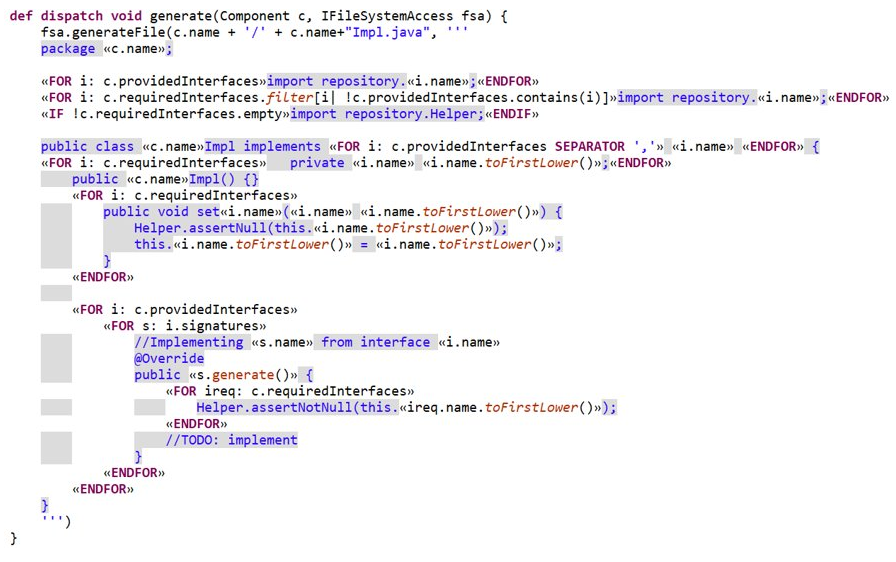
\includegraphics[height=60mm]{figures/xtend.png}
		\end{contentblock}
		\column{.5\textwidth}
		\begin{contentblock}{}
			\begin{itemize}
				\item Beispielhafte Erzeugung des Quellcodes für die DBCacheImpl-Datei mit Attributen und Methoden-Templates
				\item Generierung von \texttt{DBCache/DBCacheImpl.java}
			\end{itemize}
		\end{contentblock}
	\end{columns}
\end{frame}

\begin{frame}{Entwurfsentscheidungen bei der Code-Generierung}
	\begin{enumerate}
		\item Erzeugung der Klassen in siblings-Packages anstatt in respository-Package 
	\end{enumerate}
\end{frame}

\begin{frame}{Probleme bei der Code-Generierung}
	\begin{enumerate}
			\item OCL Constraints konnten nicht aufgelöst werden
			\begin{itemize}
				\item Deaktivierung der OCL-Validierungq
			\end{itemize} 
	\end{enumerate}
\end{frame}